\documentclass{ivoa} 
\input tthdefs
\input gitmeta

\usepackage{listings}
\lstloadlanguages{XML,SQL}
\lstset{flexiblecolumns=true,tagstyle=\ttfamily,
showstringspaces=False}
\usepackage{todonotes}

\ivoagroup{Registry}

\author[http://www.ivoa.net/cgi-bin/twiki/bin/view/IVOA/MarkusDemleitner]{Markus
Demleitner}
\author[http://www.ivoa.net/cgi-bin/twiki/bin/view/IVOA/PatrickDowler]{Patrick
Dowler}
\author[http://www.ivoa.net/cgi-bin/twiki/bin/view/IVOA/RayPlante]{Ray
Plante}
\author[http://www.ivoa.net/cgi-bin/twiki/bin/view/IVOA/GuyRixon]{Guy
Rixon}
\author[http://www.ivoa.net/cgi-bin/twiki/bin/view/IVOA/MarkTaylor]{Mark
Taylor}

\editor{Markus Demleitner}

\previousversion[http://www.ivoa.net/documents/TAPRegExt/20120827/]{REC-1.0}
\previousversion[http://www.ivoa.net/Documents/TAPRegExt/20120208]{PR-20110727}

\title{TAPRegExt: A VOResource Schema Extension for Describing TAP Services}

\begin{document}

\begin{abstract}
This document describes an XML encoding standard for metadata about
services implementing the table access protocol TAP \citep{2019ivoa.spec.0927D},
referred to as TAPRegExt.  Instance documents are
part of the service's registry record or can be obtained from the service
itself.  They deliver information to both humans and software on the languages,
output formats, and upload methods supported by the service, as well as data
models implemented by the exposed tables, optional language features,
and certain limits enforced by the service.
\end{abstract}


\section{Introduction}

\label{introduction}

The Table Access Protocol TAP \citep{2019ivoa.spec.0927D} allows
VO clients to send queries to remote database servers and receive the
results in standard formats.  In addition, it defines means to discover
database schemata on the remote side, to upload data from the local disk
or third-party hosts, and more.  TAP builds upon a variety of other
standards, premier among which is the Universal Worker Service 
\citep{2016ivoa.spec.1024H}, which describes how client and server
can negotiate the execution of a query and the retrieval of results
without having to maintain a continuous connection.

To accommodate a wide variety of requirements, the TAP specification
offers implementors many choices on optional features, resource limits, or
locally defined functionality.  One purpose of TAPRegExt is to allow the
service to communicate such choices to remote clients using the mechanisms
laid down in the VO Service Interfaces standard
\citep{2017ivoa.spec.0524G}.

Clients also need to discover TAP services offering certain kinds of data.
Central to this is the concept of a registry in which resources can be
described and consequently discovered by users and applications in the VO.
Registries receive resource descriptions as defined in the IVOA standard 
\citep{2018ivoa.spec.0625P}. In this schema, support for 
a standard service protocol is described as a service's capability; the
associated metadata is contained within the service resource description's
\texttt{<capability>} element.

TAPRegExt defines this capability element for TAP services.  In the context
of registering TAP services, an important role filled by TAPRegExt is the 
communication of supported data models to the registry.


\subsection{TAPRegExt within the VO Architecture}

\label{architecture}

\begin{figure}[th]
\begin{center}
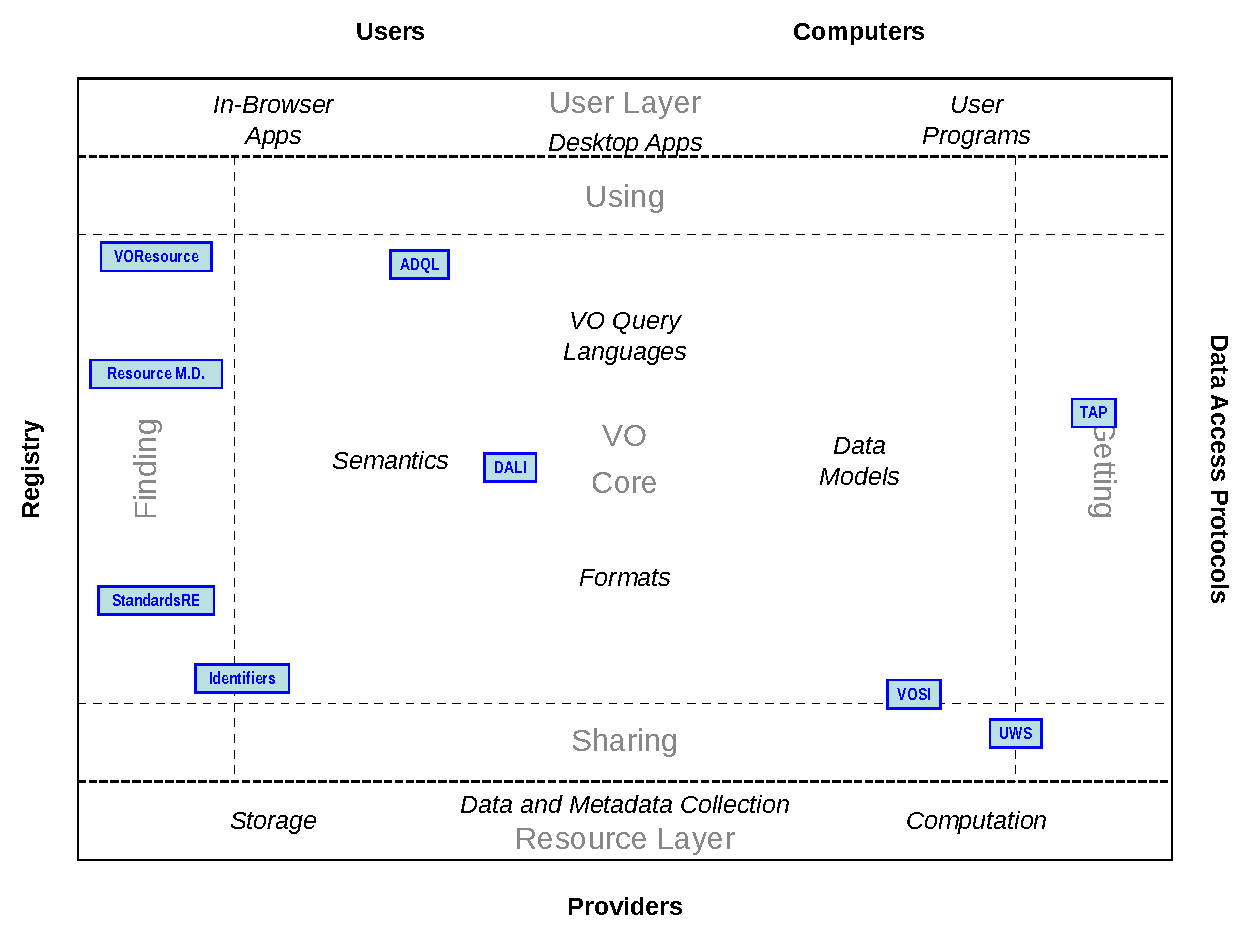
\includegraphics[width=0.9\textwidth]{role_diagram.pdf}
\end{center}
\caption{IVOA Architecture diagram with TAPRegExt and
the related standards marked up}
\label{fig:arch}
\end{figure}

This specification directly relates to other IVOA standards in the following
ways:


\begin{description}
\item[VOResource, v1.1 \citep{2018ivoa.spec.0625P}] Descriptions of services that support TAP are encoded
using the VOResource XML schema. TAPRegExt is an extension 
of the VOResource core schema.
\item[TAP, v1.1 \citep{2019ivoa.spec.0927D}]The TAP standard defines some of the concepts that TAPRegExt
deals with. The TAP standard document indirectly
refers to this document in the specification of its capabilities endpoint.
\item[UWS, v1.1 \citep{2016ivoa.spec.1024H}]The UWS standard describes additional parameters the choices 
of which are communicated using TAPRegExt.
\item[StandardsRegExt \citep{2012ivoa.spec.0508H}] TAPRegExt uses the StandardKeyEnumeration mechanism introduced
in StandardsRegExt to define controlled vocabularies.

\end{description}

This standard also relates to other IVOA standards:


\begin{description}
\item[IVOA Support Interfaces, v1.1 \citep{2017ivoa.spec.0524G}] \hfil\break VOSI describes the standard interfaces to discover metadata about
services; this document defines the response TAP services should
provide on the \texttt{capabilities} endpoint described by VOSI.
\item[IVOA defined data models]Data models specified by the IVOA can define the structure of
database tables holding instances of those data models.
The first examples of such definitions are ObsCore
\citep{2017ivoa.spec.0509L} and RegTAP \citep{2019ivoa.spec.1011D}.  Services providing
access to such tables
declare that fact within TAPRegExt instance documents.

\end{description}


\section{The Extension}

\label{taextension}

\subsection{The Schema Namespace and Location}

\label{nsloc}

The namespace associated with the TAPRegExt VOResource extension is

$$
\mbox{\texttt{http://www.ivoa.net/xml/TAPRegExt/v1.0}.}
$$

The namespace is unchanged from version 1.0 of this standard as no
changes that could break clients are introduced.

Just like the namespace URI for the VOResource schema, the
TAPRegExt namespace URI can be interpreted as a URL.  Resolving it
returns the current XML schema document
that defines the TAPRegExt schema (cf.~Appendix~\ref{app:fullschema}).

Authors of VOResource instance documents may choose to
provide a location for the VOResource XML schema document and its
extensions using the
\xmlel{xsi:schemaLocation} attribute.  
While generators are
free to provide any schema location (e.g., a local mirror), this specification
recommends using the TAPRegExt namespace URI as its location URL,
as in,


\begin{verbatim}
xsi:schemaLocation="http://www.ivoa.net/xml/TAPRegExt/v1.0
                    http://www.ivoa.net/xml/TAPRegExt/v1.0"
\end{verbatim}

Note that you must give the \texttt{xsi:schemaLocation} of
the TAPRegExt schema when the capability defined here is part of a published
registry resource record as per the IVOA Registry Interface standard 
\citep{2018ivoa.spec.0723D}.  This does not apply to the use
in a TAP server's capabilities endpoint.


\subsection{Declaring Instantiated Data Models}

\label{dms}

The IVOA defines certain data models that can be instantiated in database
tables exposed by a TAP service.  This allows a query built exclusively
on a data model or a set of data models to work on all TAP services exposing
tables instantiating the data model(s).

In TAPRegExt, a data model is identified by its IVOA identifier
\citep{2016ivoa.spec.0523D}.  The example document in Appendix~\ref{app:example}
uses this to define support for both the ObsCore and RegTAP data models.

% GENERATED: !schemadoc TAPRegExt-v1.1.xsd DataModelType
\begin{generated}
\begingroup
      	\renewcommand*\descriptionlabel[1]{%
      	\hbox to 5.5em{\emph{#1}\hfil}}\vspace{2ex}\noindent\textbf{\xmlel{tr:DataModelType} Type Schema Documentation}

\noindent{\small
        An IVOA defined data model, identified by an IVORN 
        intended for machine consumption and a short label
        intended for human comsumption.
      \par}

\vspace{1ex}\noindent\textbf{\xmlel{tr:DataModelType} Type Schema Definition}

\begin{lstlisting}[language=XML,basicstyle=\footnotesize]
<xs:complexType name="DataModelType" >
  <xs:simpleContent >
    <xs:extension base="xs:token" >
      <xs:attribute name="ivo-id" type="xs:anyURI" use="required" />
    </xs:extension>
  </xs:simpleContent>
</xs:complexType>
\end{lstlisting}

\vspace{0.5ex}\noindent\textbf{\xmlel{tr:DataModelType} Attributes}

\begingroup\small\begin{bigdescription}
\item[ivo-id]
\begin{description}
\item[Type] a URI: \xmlel{xs:anyURI}
\item[Meaning] 
            The IVOID of the data model.
            
\item[Occurrence] required
\end{description}


\end{bigdescription}\endgroup

\endgroup
\end{generated}

% /GENERATED

\subsection{Languages Supported}

\label{langs}

TAP services may offer a variety of query languages.  In TAPRegExt, the
\xmlel{language} element allows the communication of what languages are
available on a service.  TAP defines values of the \texttt{LANG} parameter
to have either the form \texttt{<name>-<version>} or the form
\texttt{<name>}, where the latter form leaves the choice of the
version to the server.  Therefore, a language is defined using a name and one
or more versions.

The recommended way to associate larger amounts of documentation with a
language entry in a capability element is via registration of the language
using the mechanisms defined in StdRegExt \citep{2012ivoa.spec.0508H} and associating
the registry record with the language element through the latter's 
\xmlel{ivo-id}
attribute.  The IVOID for the only language mandatory for TAP services,
ADQL 2.0, is 
\nolinkurl{ivo://ivoa.net/std/ADQL#v2.0}.
.

The type of the \xmlel{ivo-id} attribute on version is 
\xmlel{xs:anyURI} as opposed to \xmlel{vr:IdentifierURI} since
the latter does not allow fragment identifiers in VOResource 1.0. 
The description constrains the value to be an
IVOID (i.e., a URI with a schema of ivo:), though.  
The same reasoning applies to the \xmlel{ivo-id}
attributes of \xmlel{outputFormat} and \xmlel{uploadMethod}.

% GENERATED: !schemadoc TAPRegExt-v1.1.xsd Language
\begin{generated}
\begingroup
      	\renewcommand*\descriptionlabel[1]{%
      	\hbox to 5.5em{\emph{#1}\hfil}}\vspace{2ex}\noindent\textbf{\xmlel{tr:Language} Type Schema Documentation}

\noindent{\small
      A query language supported by the service.
      \par}

\noindent{\small
      Each language element can describe one or more versions
      of a language.  Either name alone or name-version can be
      used as values for the server's LANG parameter.
      \par}

\vspace{1ex}\noindent\textbf{\xmlel{tr:Language} Type Schema Definition}

\begin{lstlisting}[language=XML,basicstyle=\footnotesize]
<xs:complexType name="Language" >
  <xs:sequence >
    <xs:element name="name" type="xs:NCName" />
    <xs:element name="version" type="tr:Version" minOccurs="1"
              maxOccurs="unbounded" />
    <xs:element name="description" type="xs:token" minOccurs="0" />
    <xs:element name="languageFeatures"
              type="tr:LanguageFeatureList"
              minOccurs="0"
              maxOccurs="unbounded" />
  </xs:sequence>
</xs:complexType>
\end{lstlisting}

\vspace{0.5ex}\noindent\textbf{\xmlel{tr:Language} Metadata Elements}

\begingroup\small\begin{bigdescription}\item[Element \xmlel{name}]
\begin{description}
\item[Type] a prefixless XML name
\item[Meaning] 
          The name of the language without a version suffix.
          
\item[Occurrence] required

\end{description}
\item[Element \xmlel{version}]
\begin{description}
\item[Type] a string with optional attributes
\item[Meaning] 
            A version of the language supported by the server.
          
\item[Occurrence] required; multiple occurrences allowed.

\end{description}
\item[Element \xmlel{description}]
\begin{description}
\item[Type] string: \xmlel{xs:token}
\item[Meaning] 
          A short, human-readable description of the
          query language.
          
\item[Occurrence] optional

\end{description}
\item[Element \xmlel{languageFeatures}]
\begin{description}
\item[Type] composite: \xmlel{tr:LanguageFeatureList}
\item[Meaning] 
            Optional features of the query language, grouped by
            feature type.
          
\item[Occurrence] optional; multiple occurrences allowed.
\item[Comment] 
            This includes listing user defined functions, geometry support,
            or similar concepts.
          

\end{description}


\end{bigdescription}\endgroup

\endgroup
\end{generated}

% /GENERATED

% GENERATED: !schemadoc TAPRegExt-v1.1.xsd Version
\begin{generated}
\begingroup
      	\renewcommand*\descriptionlabel[1]{%
      	\hbox to 5.5em{\emph{#1}\hfil}}\vspace{2ex}\noindent\textbf{\xmlel{tr:Version} Type Schema Documentation}

\noindent{\small
      One version of the language supported by the service.
      \par}

\noindent{\small
      If the service supports more than one version of the
      language, include multiple version elements.
      It is recommended that you use a version numbering
      scheme like MAJOR.MINOR in such a way that sorting
      by ascending character codes will leave the most
      recent version at the bottom of the list.
      \par}

\vspace{1ex}\noindent\textbf{\xmlel{tr:Version} Type Schema Definition}

\begin{lstlisting}[language=XML,basicstyle=\footnotesize]
<xs:complexType name="Version" >
  <xs:simpleContent >
    <xs:extension base="xs:token" >
      <xs:attribute name="ivo-id" type="xs:anyURI" />
    </xs:extension>
  </xs:simpleContent>
</xs:complexType>
\end{lstlisting}

\vspace{0.5ex}\noindent\textbf{\xmlel{tr:Version} Attributes}

\begingroup\small\begin{bigdescription}
\item[ivo-id]
\begin{description}
\item[Type] a URI: \xmlel{xs:anyURI}
\item[Meaning] 
            An optional IVOID of the language.
            
\item[Occurrence] optional
\item[Comment] 
              To more formally define a language supported by a service,
              a resource record for the language can be created, either
              centrally on the Registry of Registries or by other registry operators.  
              When such a record exists, the ivo-id attribute of language
              should point to it.
            
\end{description}


\end{bigdescription}\endgroup

\endgroup
\end{generated}

% /GENERATED


Query languages may support optional features.  For ADQL, the most prominent
of those are user-defined functions, i.e., functions not defined in the language
standard but added by the operators of the service, and geometry functions.
Such optional features may be communicated to the service client in
\xmlel{tr:languageFeatures} elements.  

Each such list is labelled with a \xmlel{type} attribute
indicating the type of language option being described.
This string should be an IVOID whose semantics in this context,
along with the semantics of the content of its descendant 
\xmlel{feature/form} elements,
can be documented in association with the language in question.

TAPRegExt itself defines the following feature types:


\begin{bigdescription}
\item[\nolinkurl{ivo://ivoa.net/std/TAPRegExt\#features-udf}] Each feature declares a user-defined ADQL (or similar) function supported.
    The content of the \xmlel{form} element
    must be the signature of the function, written to match the
    \texttt{signature} nonterminal in the following grammar:


\begin{verbatim}
signature ::= <funcname> <arglist> "->" <type_name>
funcname  ::= <regular_identifier>
arglist   ::= "(" <arg> { "," <arg> } ")"
arg       ::= <regular_identifier> <type_name>
\end{verbatim}

The \texttt{type\_name} nonterminal is not defined by the ADQL
		grammar in version 2.0. 
		For the purposes of TAPRegExt, it is sufficient to assume
		it expands to ``some sort of SQL type specifier'' (which may
		include spaces and parentheses).  For an enumeration of common types
		in ADQL, refer to the last column of the table in section 2.5 of 
		the TAP standard \citep{2019ivoa.spec.0927D}.

Example:


\begin{lstlisting}[language=XML,basicstyle=\footnotesize]
<languageFeatures type="ivo://ivoa.net/std/TAPRegExt#features-udf">
  <feature>
    <form>match(pattern TEXT, string TEXT) -> INTEGER</form>
    <description>
      match returns 1 if the POSIX regular expression pattern 
      matches anything in string, 0 otherwise.
    </description>
  </feature>
</languageFeatures>
\end{lstlisting}


\item[\nolinkurl{ivo://ivoa.net/std/TAPRegExt\#features-adqlgeo}] Each feature declares support for one of the geometry functions 
		defined by ADQL
    (support for these functions is in general optional for ADQL
    implementations, though TAP imposes some constraints on what 
    combinations of support are permitted).

The signature of these functions, where supported, is fixed by ADQL;
    the content of the \xmlel{form} element
    is just the name of the function.

Example:


\begin{lstlisting}[language=XML,basicstyle=\footnotesize]
<feature>
  <form>CONTAINS</form>
</feature>
\end{lstlisting}



\end{bigdescription}


% GENERATED: !schemadoc TAPRegExt-v1.1.xsd LanguageFeatureList
\begin{generated}
\begingroup
      	\renewcommand*\descriptionlabel[1]{%
      	\hbox to 5.5em{\emph{#1}\hfil}}\vspace{2ex}\noindent\textbf{\xmlel{tr:LanguageFeatureList} Type Schema Documentation}

\noindent{\small
        An enumeration of non-standard or non-mandatory features of 
        a specific type implemented by the language.
      \par}

\noindent{\small
        A feature type is a language-dependent concept like 
        "user defined function", "geometry support", or possibly 
        "units supported".  A featureList gives all features of
        a given type applicable for the service.  Multiple featureLists
        are possible.

        All feature in a given list are of the same type.  This type
        is declared using the mandatory type attribute,
        the value of which will typically be an IVOID.
        To see values defined in TAPRegExt,
        retrieve the ivo://ivoa.net/std/TAPRegExt
        resource record and look for keys starting with "features-".
      \par}

\vspace{1ex}\noindent\textbf{\xmlel{tr:LanguageFeatureList} Type Schema Definition}

\begin{lstlisting}[language=XML,basicstyle=\footnotesize]
<xs:complexType name="LanguageFeatureList" >
  <xs:sequence >
    <xs:element name="feature" type="tr:LanguageFeature" minOccurs="0"
              maxOccurs="unbounded" />
  </xs:sequence>
  <xs:attribute name="type" type="xs:anyURI" use="required" />
</xs:complexType>
\end{lstlisting}

\vspace{0.5ex}\noindent\textbf{\xmlel{tr:LanguageFeatureList} Attributes}

\begingroup\small\begin{bigdescription}
\item[type]
\begin{description}
\item[Type] a URI: \xmlel{xs:anyURI}
\item[Meaning] 
          The type of the features given here.
        
\item[Occurrence] required
\item[Comment] 
          This is in general an IVOID.  TAPRegExt itself gives
          IVOIDs for defining user defined functions and geometry
          support.
        
\end{description}


\end{bigdescription}\endgroup



\vspace{0.5ex}\noindent\textbf{\xmlel{tr:LanguageFeatureList} Metadata Elements}

\begingroup\small\begin{bigdescription}\item[Element \xmlel{feature}]
\begin{description}
\item[Type] composite: \xmlel{tr:LanguageFeature}
\item[Meaning] 
            A language feature of the type given by the
            type attribute.
          
\item[Occurrence] optional; multiple occurrences allowed.

\end{description}


\end{bigdescription}\endgroup

\endgroup
\end{generated}

% /GENERATED

% GENERATED: !schemadoc TAPRegExt-v1.1.xsd LanguageFeature
\begin{generated}
\begingroup
      	\renewcommand*\descriptionlabel[1]{%
      	\hbox to 5.5em{\emph{#1}\hfil}}\vspace{2ex}\noindent\textbf{\xmlel{tr:LanguageFeature} Type Schema Documentation}

\noindent{\small
        A non-standard or non-mandatory feature implemented
        by the language..
      \par}

\vspace{1ex}\noindent\textbf{\xmlel{tr:LanguageFeature} Type Schema Definition}

\begin{lstlisting}[language=XML,basicstyle=\footnotesize]
<xs:complexType name="LanguageFeature" >
  <xs:sequence >
    <xs:element name="form" type="xs:token" />
    <xs:element name="description" type="xs:string" minOccurs="0" />
  </xs:sequence>
</xs:complexType>
\end{lstlisting}

\vspace{0.5ex}\noindent\textbf{\xmlel{tr:LanguageFeature} Metadata Elements}

\begingroup\small\begin{bigdescription}\item[Element \xmlel{form}]
\begin{description}
\item[Type] string: \xmlel{xs:token}
\item[Meaning] 
            Formal notation for the language feature.
          
\item[Occurrence] required
\item[Comment] 
            The syntax for the content of this element is defined by the
            type attribute of its parent language list.
          

\end{description}
\item[Element \xmlel{description}]
\begin{description}
\item[Type] string: \xmlel{xs:string}
\item[Meaning] 
            Human-readable freeform documentation for the language feature.
          
\item[Occurrence] optional

\end{description}


\end{bigdescription}\endgroup

\endgroup
\end{generated}

% /GENERATED

\subsection{Output Formats}

\label{outforms}

A TAP service may offer a variety of output formats.
What output formats are available is defined using
\xmlel{outputFormat} elements.   They 
declare an RFC 2046 media type \citep{std:MIME} as well
as aliases (the shorthand forms the server also accepts in the 
FORMAT parameter).  If desired, the format can be further described with an
IVOID in the ivo-id attribute; TAPRegExt provides keys for some variants of
VOTables which are not interoperably distinguishable by their MIME types so far:


\begin{description}
\item[\normalfont\texttt{output-votable-td}]A VOTable in which all DATA elements contain a TABLEDATA element
\item[\normalfont\texttt{output-votable-binary}]A VOTable in which all DATA elements contain a STREAM element
	with a BINARY child
\item[\normalfont\texttt{output-votable-binary2}]A VOTable in which all DATA elements contain a STREAM element
	with a BINARY2 child
\end{description}

% GENERATED: !schemadoc TAPRegExt-v1.1.xsd OutputFormat
\begin{generated}
\begingroup
      	\renewcommand*\descriptionlabel[1]{%
      	\hbox to 5.5em{\emph{#1}\hfil}}\vspace{2ex}\noindent\textbf{\xmlel{tr:OutputFormat} Type Schema Documentation}

\noindent{\small
      An output format supported by the service.
      \par}

\noindent{\small
      All TAP services must support VOTable output, with media types as 
      requested by the FORMAT parameter if applicable (cf.~section 2.7.1 
      of the TAP standard).

      The primary identifier for an output format is the RFC 2046 media
      type.  If you want to register an output format, you must
      use a media type (or make one up using the x- syntax), although
      the concrete media syntax is not enforced by the schema.

      For more detailed specification, an IVOID may be used.
      \par}

\vspace{1ex}\noindent\textbf{\xmlel{tr:OutputFormat} Type Schema Definition}

\begin{lstlisting}[language=XML,basicstyle=\footnotesize]
<xs:complexType name="OutputFormat" >
  <xs:sequence >
    <xs:element name="mime" type="xs:token" />
    <xs:element name="alias" type="xs:token" minOccurs="0"
              maxOccurs="unbounded" />
  </xs:sequence>
  <xs:attribute name="ivo-id" type="xs:anyURI" />
</xs:complexType>
\end{lstlisting}

\vspace{0.5ex}\noindent\textbf{\xmlel{tr:OutputFormat} Attributes}

\begingroup\small\begin{bigdescription}
\item[ivo-id]
\begin{description}
\item[Type] a URI: \xmlel{xs:anyURI}
\item[Meaning] 
        An optional IVOID of the output format.
        
\item[Occurrence] optional
\item[Comment] 
          When the media type does not uniquely define the
          format (or a generic media type like application/octet-stream or
          text/plain is given), the IVOID can point to a key
          or StandardsRegExt document defining the format more
          precisely.  To see values defined in TAPRegExt,
          retrieve the ivo://ivoa.net/std/TAPRegExt
          resource record and look for keys starting with {"}output-{"}.
        
\end{description}


\end{bigdescription}\endgroup



\vspace{0.5ex}\noindent\textbf{\xmlel{tr:OutputFormat} Metadata Elements}

\begingroup\small\begin{bigdescription}\item[Element \xmlel{mime}]
\begin{description}
\item[Type] string: \xmlel{xs:token}
\item[Meaning] 
          The media type of this format.
          
\item[Occurrence] required
\item[Comment] 
          The format of this string is specified by RFC 2046.
          The service has to accept this string as a 
          value of the FORMAT parameter.
          

\end{description}
\item[Element \xmlel{alias}]
\begin{description}
\item[Type] string: \xmlel{xs:token}
\item[Meaning] 
          Other values of FORMAT ({"}shorthands{"}) that make the service return 
          documents with the media type.
          
\item[Occurrence] optional; multiple occurrences allowed.

\end{description}


\end{bigdescription}\endgroup

\endgroup
\end{generated}

% /GENERATED

\subsection{Upload Methods}

\label{uploadmethods}

TAP services should allow the upload of VOTables.  They can support
various methods to do this: HTTP upload, retrieval by URL, but also VOSpace
or possibly retrieval using Grid protocols.  Since an actual specification
of the details of such protocols is far beyond the scope of a registry
document and probably would not benefit clients anyway, the upload
methods are given as IVOIDs.

IVOIDs for the standard upload methods are provided within the
resource record
\texttt{ivo://ivoa.net/std/TAPRegExt}.  
The IVOIDs are built by using the keys as fragments after the 
TAPRegExt IVOID.

It is permitted to register upload methods under authorities other than
ivoa.net.
The registry records can then provide more in-depth information. For
the upload methods defined in the TAP specification, however, 
the IVOIDs of the keys in the TAPRegExt resource record must be used to enable
clients to identify supported methods using string comparisons.

This document defines the following protocol identifiers:


\begin{itemize}

\item \texttt{upload-inline} -- HTTP upload as per section 2.5.2 of 
the TAP standard \citep{2019ivoa.spec.0927D}.{}

\item \texttt{upload-http} -- retrieval from an http URL.{}

\item \texttt{upload-https} -- retrieval from an https URL.{}

\item \texttt{upload-ftp} -- retrieval from an ftp URL.{}

\end{itemize}

Thus, a service offering upload by retrieving from ftp and http URLs
would say:


\begin{lstlisting}[language=XML,basicstyle=\footnotesize]
  <uploadMethod ivo-id="ivo://ivoa.net/std/TAPRegExt#upload-http"/>
  <uploadMethod ivo-id="ivo://ivoa.net/std/TAPRegExt#upload-ftp"/>
\end{lstlisting}

% GENERATED: !schemadoc TAPRegExt-v1.1.xsd UploadMethod
\begin{generated}
\begingroup
      	\renewcommand*\descriptionlabel[1]{%
      	\hbox to 5.5em{\emph{#1}\hfil}}\vspace{2ex}\noindent\textbf{\xmlel{tr:UploadMethod} Type Schema Documentation}

\noindent{\small
      An upload method as defined by IVOA.
      \par}

\noindent{\small
      Upload methods are always identified by an IVOID.  
      Descriptions can be obtained by dereferencing this
      IVOID.  To see values defined in TAPRegExt,
      retrieve the ivo://ivoa.net/std/TAPRegExt
      resource record and look for keys starting with "upload-".

      You can register custom upload methods, but you must use the
      standard IVOIDs for the upload methods defined in the TAP
      specification.
      \par}

\vspace{1ex}\noindent\textbf{\xmlel{tr:UploadMethod} Type Schema Definition}

\begin{lstlisting}[language=XML,basicstyle=\footnotesize]
<xs:complexType name="UploadMethod" >
  <xs:complexContent >
    <xs:restriction base="xs:anyType" >
      <xs:attribute name="ivo-id" type="xs:anyURI" />
    </xs:restriction>
  </xs:complexContent>
</xs:complexType>
\end{lstlisting}

\vspace{0.5ex}\noindent\textbf{\xmlel{tr:UploadMethod} Attributes}

\begingroup\small\begin{bigdescription}
\item[ivo-id]
\begin{description}
\item[Type] a URI: \xmlel{xs:anyURI}
\item[Meaning] 
            The IVOID of the upload method.
            
\item[Occurrence] optional
\end{description}


\end{bigdescription}\endgroup

\endgroup
\end{generated}

% /GENERATED

\subsection{Resource Limits}

\label{reslimits}

TAP services usually impose certain limits on resource usage by clients,
e.g., a maximum run time per query, or a maximum number of rows in the result
set.  Services assign such limits to newly created jobs and may
allow raising the limits by means of queries or query parameters (e.g., the
size of the result set is limited by the \texttt{MAXREC} parameter, whereas
the date of job destruction may be changed by posting to the
\texttt{destruction} parameter).  Services may put some limit to how
far the resource limitations may be raised.

TAPRegExt's \xmlel{capabilities} element allows the declaration of such limits.
These declarations are primarily intended for human consumption and should give
conservative guidelines.  Thus, the operators of a service implementing a
complex, possibly dynamic limits policy should give lower estimates here.

If a service supports authentication and has different
limits depending on what user is authenticated, it should make an effort
to guess the limits applying to a given client (e.g., when
authentication tokens are present in the request).  Limits reported to
the Registry should reflect limits for unauthenticated use unless the
service does not admit unauthenticated requests.

The resource limits applying to newly created jobs are given in
\xmlel{default} elements, the limits beyond which users cannot
raise the limits are given in \xmlel{hard} elements.

Note that the absence of a specification of limits does not imply that
no limits are enforced.


\subsubsection{Limits on Time}
This document defines two time-like resource limits:


\begin{itemize}

\item \xmlel{retentionPeriod} -- the time from job creation until
		\texttt{destruction}.{}

\item \xmlel{executionDuration} -- the maximal run time given to
		a query.{}

\end{itemize}
All values in time-like limits are given in seconds.  Both 
\xmlel{retentionPeriod} and \xmlel{executionDuration} are of type
\xmlel{tr:TimeLimits}.

% GENERATED: !schemadoc TAPRegExt-v1.1.xsd TimeLimits
\begin{generated}
\begingroup
      	\renewcommand*\descriptionlabel[1]{%
      	\hbox to 5.5em{\emph{#1}\hfil}}\vspace{2ex}\noindent\textbf{\xmlel{tr:TimeLimits} Type Schema Documentation}

\noindent{\small
      Time-valued limits, all values given in seconds.
      \par}

\vspace{1ex}\noindent\textbf{\xmlel{tr:TimeLimits} Type Schema Definition}

\begin{lstlisting}[language=XML,basicstyle=\footnotesize]
<xs:complexType name="TimeLimits" >
  <xs:sequence >
    <xs:element name="default" type="xs:integer" minOccurs="0"
              maxOccurs="1" />
    <xs:element name="hard" type="xs:integer" minOccurs="0" maxOccurs="1" />
  </xs:sequence>
</xs:complexType>
\end{lstlisting}

\vspace{0.5ex}\noindent\textbf{\xmlel{tr:TimeLimits} Metadata Elements}

\begingroup\small\begin{bigdescription}\item[Element \xmlel{default}]
\begin{description}
\item[Type] integer
\item[Meaning] 
          The value of this limit for newly-created jobs, given in seconds.
          
\item[Occurrence] optional

\end{description}
\item[Element \xmlel{hard}]
\begin{description}
\item[Type] integer
\item[Meaning] 
          The value this limit cannot be raised above, given in seconds.
          
\item[Occurrence] optional

\end{description}


\end{bigdescription}\endgroup

\endgroup
\end{generated}

% /GENERATED

\subsubsection{Limits on Data}
Limits on data are expressed much like time limits in that they give
\xmlel{default} and a \xmlel{hard} value as well.  
Both those values have a unit attribute that can either be \texttt{byte}
or \texttt{row} for data limits.

This document defines two resource limits on data:


\begin{itemize}

\item \xmlel{outputLimit} -- if \xmlel{unit} is \texttt{row} here,
the \xmlel{default} gives the
value of TAP's \texttt{MAXREC} parameter the service will use when none
is specified.{}

\item \xmlel{uploadLimit} -- the maximum size of uploads.  This 
is not a TAP adjustable parameter.  The \xmlel{default} value
advises clients about the server's wishes as to a limit above which
some sort of acknowledgement should be requested from the user.  The 
\xmlel{hard} limit gives the maximum size of an upload to the 
server.{}

\end{itemize}
Data limits are defined using the \xmlel{tr:DataLimits}
and \xmlel{tr:DataLimit} types:


% GENERATED: !schemadoc TAPRegExt-v1.1.xsd DataLimits
\begin{generated}
\begingroup
      	\renewcommand*\descriptionlabel[1]{%
      	\hbox to 5.5em{\emph{#1}\hfil}}\vspace{2ex}\noindent\textbf{\xmlel{tr:DataLimits} Type Schema Documentation}

\noindent{\small
      Limits on data sizes, given in rows or bytes.
      \par}

\vspace{1ex}\noindent\textbf{\xmlel{tr:DataLimits} Type Schema Definition}

\begin{lstlisting}[language=XML,basicstyle=\footnotesize]
<xs:complexType name="DataLimits" >
  <xs:sequence >
    <xs:element name="default" type="tr:DataLimit" minOccurs="0"
              maxOccurs="1" />
    <xs:element name="hard" type="tr:DataLimit" minOccurs="0"
              maxOccurs="1" />
  </xs:sequence>
</xs:complexType>
\end{lstlisting}

\vspace{0.5ex}\noindent\textbf{\xmlel{tr:DataLimits} Metadata Elements}

\begingroup\small\begin{bigdescription}\item[Element \xmlel{default}]
\begin{description}
\item[Type] an integer with optional attributes
\item[Meaning] 
          The value of this limit for newly-created jobs.
          
\item[Occurrence] optional

\end{description}
\item[Element \xmlel{hard}]
\begin{description}
\item[Type] an integer with optional attributes
\item[Meaning] 
          The value this limit cannot be raised above.
          
\item[Occurrence] optional

\end{description}


\end{bigdescription}\endgroup

\endgroup
\end{generated}

% /GENERATED

% GENERATED: !schemadoc TAPRegExt-v1.1.xsd DataLimit
\begin{generated}
\begingroup
      	\renewcommand*\descriptionlabel[1]{%
      	\hbox to 5.5em{\emph{#1}\hfil}}\vspace{2ex}\noindent\textbf{\xmlel{tr:DataLimit} Type Schema Documentation}

\noindent{\small
      A limit on some data size, either in rows or in bytes.
      \par}

\vspace{1ex}\noindent\textbf{\xmlel{tr:DataLimit} Type Schema Definition}

\begin{lstlisting}[language=XML,basicstyle=\footnotesize]
<xs:complexType name="DataLimit" >
  <xs:simpleContent >
    <xs:extension base="xs:integer" >
      <xs:attribute name="unit" use="required" >
        <xs:simpleType >
          <xs:restriction base="xs:token" >
            <xs:enumeration value="byte" />
            <xs:enumeration value="row" />
          </xs:restriction>
        </xs:simpleType>
      </xs:attribute>
    </xs:extension>
  </xs:simpleContent>
</xs:complexType>
\end{lstlisting}

\vspace{0.5ex}\noindent\textbf{\xmlel{tr:DataLimit} Attributes}

\begingroup\small\begin{bigdescription}
\item[unit]
\begin{description}
\item[Type] string with controlled vocabulary
\item[Meaning] 
            The unit of the limit specified.
            
\item[Occurrence] required

\item[Allowed Values]\hfil
\begin{longtermsdescription}\item[byte]
\item[row]
\end{longtermsdescription}
\end{description}


\end{bigdescription}\endgroup

\endgroup
\end{generated}

% /GENERATED

\subsection{Interface Declaration}
\label{intfdecl}

Version 1.0 of this specification used a VODataService
\xmlel{vs:ParamHTTP} interface to declare the TAP service's base URL.
This was mainly done to maintain common service discovery patterns --
other DAL protocols use \xmlel{vs:ParamHTTP}-typed interfaces as well
--, but it ignored the semantics of the type, which in particular is
that the access URL of such an interface is what clients use in queries.
Against that, the TAP specification actually leaves open what
directly dereferencing the base URL should result in.  Instead, all
functionality is offered through children of the base URL.  The abuse of
\xmlel{vs:ParamHTTP} later had a severe fallout as discussed in
\citet{note:caproles}.

However, existing TAP clients rely on the interface declaration for
discovery, and hence all
capability elements with a TAPRegExt version~1 \xmlel{standardID} must include
a \xmlel{vs:ParamHTTP}-typed interface with

\begin{itemize}
\item a child element \xmlel{accessURL} with its content the base URL of
the TAP service (the parent of sync, async, etc.) and its \xmlel{use}
attribute set to \verb|base|.
\item its \xmlel{role} attribute set to \verb|std|
\item its \xmlel{version} attribute set to the version of the TAP
specification implemented.
\end{itemize}

In order to open the path to advanced use cases (e.g., involving
authenticated access), services implementing TAPRegExt~1.1 must include
another interface element of type \xmlel{tr:DALIInterface}.  

% GENERATED: !schemadoc TAPRegExt-v1.1.xsd DALIInterface
\begin{generated}
\begingroup
      	\renewcommand*\descriptionlabel[1]{%
      	\hbox to 5.5em{\emph{#1}\hfil}}\vspace{2ex}\noindent\textbf{\xmlel{tr:DALIInterface} Type Schema Documentation}

\noindent{\small
        An interface for a complex, multi-endpoint interfaces as
        regulated by DALI.
      \par}

\noindent{\small
        In addition to the standard vr:Interface elements, DALIInterfaces
        have endpoints, listed by name; that name doubles as a path segment
        to append to the interface's access URL, yielding the URI at
        which the endpoint is operated.
      \par}

\vspace{1ex}\noindent\textbf{\xmlel{tr:DALIInterface} Type Schema Definition}

\begin{lstlisting}[language=XML,basicstyle=\footnotesize]
<xs:complexType name="DALIInterface" >
  <xs:complexContent >
    <xs:extension base="vr:Interface" >
      <xs:sequence >
        <xs:element name="endpoint" type="tr:Endpoint" minOccurs="0"
                  maxOccurs="unbounded" />
      </xs:sequence>
    </xs:extension>
  </xs:complexContent>
</xs:complexType>
\end{lstlisting}

\vspace{0.5ex}\noindent\textbf{\xmlel{tr:DALIInterface} Extension Metadata Elements}

\begingroup\small\begin{bigdescription}\item[Element \xmlel{endpoint}]
\begin{description}
\item[Type] composite: \xmlel{tr:Endpoint}
\item[Meaning] 
                An endpoint accessible through this interface.
              
\item[Occurrence] optional; multiple occurrences allowed.

\end{description}


\end{bigdescription}\endgroup

\endgroup
\end{generated}

% /GENERATED

The \xmlel{tr:DALIInterface}-typed interface must satisfy the same
requirements as the \xmlel{vs:ParamHTTP}-typed one as regards its
\xmlel{accessURL} child and \xmlel{role} and \xmlel{version} attributes.
Furthermore, this interface now enumerates the various endpoints exposed
below the base URI in \xmlel{endpoint} elements\todo{We may want to
support vocab on endpoint; or do we want an implicit prefix as in
datalink?}.

% GENERATED: !schemadoc TAPRegExt-v1.1.xsd Endpoint
\begin{generated}
\begingroup
      	\renewcommand*\descriptionlabel[1]{%
      	\hbox to 5.5em{\emph{#1}\hfil}}\vspace{2ex}\noindent\textbf{\xmlel{tr:Endpoint} Type Schema Documentation}

\noindent{\small
        An endpoint of a complex interface.
      \par}

\noindent{\small
        An endpoint is characterised and addrssed by its name;
        they can further be defined through RDF triples.  This is a
        generic extension mechanism for endpoint-specific metadata,
        primarily intended for custom, vendor-specific extensions.
      \par}

\vspace{1ex}\noindent\textbf{\xmlel{tr:Endpoint} Type Schema Definition}

\begin{lstlisting}[language=XML,basicstyle=\footnotesize]
<xs:complexType name="Endpoint" >
  <xs:sequence >
    <xs:element name="name" type="xs:token" minOccurs="1" maxOccurs="1" />
    <xs:element name="meta" type="tr:MetaTriple" minOccurs="0"
              maxOccurs="unbounded" />
  </xs:sequence>
</xs:complexType>
\end{lstlisting}

\vspace{0.5ex}\noindent\textbf{\xmlel{tr:Endpoint} Metadata Elements}

\begingroup\small\begin{bigdescription}\item[Element \xmlel{name}]
\begin{description}
\item[Type] string: \xmlel{xs:token}
\item[Meaning] 
            The endpoint name, which is also the last component of the
            path of its URI.
          
\item[Occurrence] required
\item[Comment] 
            Names without dashes are reserved for IVOA use and are expected to
            work the same way on all services.  Well-known examples for
            such endpoint names include sync, async, and tables.
          

\end{description}
\item[Element \xmlel{meta}]
\begin{description}
\item[Type] a string with optional attributes
\item[Meaning] 
            Auxiliary information on this endpoint.
          
\item[Occurrence] optional; multiple occurrences allowed.

\end{description}


\end{bigdescription}\endgroup

\endgroup
\end{generated}

% /GENERATED

For TAP, at least the \verb|sync|, \verb|async|, and \verb|tables|
endpoints must be declared, as well as \verb|examples| if present.  The VOSI
capabilities URL, while in TAP also a child of the base URL,
continues to be declared in separate capability in this version rather
than a DALI interface endpoint.  TAPRegExt specifically discourages
returning different capability contents from different interfaces (e.g.,
with and without authentication) of a service.

While in general, not overly much configurability should be enabled on
the level of endpoints, operators can attach extra per-endpoint metadata
using their \xmlel{meta} children.  These support a subset of
the attributes defined by RDFa lite \citep{std:RDFaLite11}, enough to
make statements consisting of a subject (\xmlel{about}), a predicate
(\xmlel{property}), and an object (content or \xmlel{resource}):

% GENERATED: !schemadoc TAPRegExt-v1.1.xsd MetaTriple
\begin{generated}
\begingroup
      	\renewcommand*\descriptionlabel[1]{%
      	\hbox to 5.5em{\emph{#1}\hfil}}\vspace{2ex}\noindent\textbf{\xmlel{tr:MetaTriple} Type Schema Documentation}

\noindent{\small
        A container for an RDFa triple giving information related to
        an endpoint.
      \par}

\vspace{1ex}\noindent\textbf{\xmlel{tr:MetaTriple} Type Schema Definition}

\begin{lstlisting}[language=XML,basicstyle=\footnotesize]
<xs:complexType name="MetaTriple" >
  <xs:simpleContent >
    <xs:extension base="xs:token" >
      <xs:attribute name="about" type="xs:anyURI" use="optional" />
      <xs:attribute name="property" type="xs:anyURI" use="required" />
      <xs:attribute name="resource" type="xs:anyURI" use="optional" />
    </xs:extension>
  </xs:simpleContent>
</xs:complexType>
\end{lstlisting}

\vspace{0.5ex}\noindent\textbf{\xmlel{tr:MetaTriple} Attributes}

\begingroup\small\begin{bigdescription}
\item[about]
\begin{description}
\item[Type] a URI: \xmlel{xs:anyURI}
\item[Meaning] 
              The subject of the statement.
            
\item[Occurrence] optional
\item[Comment] 
              If missing, the endpoint itself is assumed as the subject.
            
\end{description}
\item[property]
\begin{description}
\item[Type] a URI: \xmlel{xs:anyURI}
\item[Meaning] 
              The property of the statement.
            
\item[Occurrence] required
\item[Comment] 
              This is a reference to an RDF resource.  IVOA standards may define
              semantics for scheme-less URI; non-IVOA properties must use
              full URIs with at least scheme and authority; in this
              version, no vocab attributes are supported.
            
\end{description}
\item[resource]
\begin{description}
\item[Type] a URI: \xmlel{xs:anyURI}
\item[Meaning] 
              The object of the statement.
            
\item[Occurrence] optional
\item[Comment] 
              If missing, the text content of the element is used as the
              object.
            
\end{description}


\end{bigdescription}\endgroup

\endgroup
\end{generated}

% /GENERATED

This is intended to give operators the possibility to communicate extra
information to custom clients primarily by defining properties, which
are simply URIs controlled by the operator and should dereference to
documents explaining the semantics of the properties, ideally authored
in HTML.  The object of the statement is typically given by the element
contents, but where the object cannot be inlined, the \xmlel{meta}'s
\xmlel{resource} attribute can be used instead.

For instance, to convey a custom method to upload tables on an
(authenticated) tables endpoint, an operator could say:

\begin{lstlisting}[language=XML, basicstyle=\footnotesize]
<endpoint>
  <name>tables</name>
  <meta property="http://operator.example.edu/supports-our-extension"
    >table-upload</meta>
</endpoint>
\end{lstlisting}

To prevent a fragmentation of the TAP standard, such extensions should
be restricted to single service providers and custom clients and be
considered for addition to the TAP standard as other parties take them
up.

Because it models the most essential aspects of RDF, the \xmlel{meta}
element, in principle, allows operators to build almost arbitrarily
complex metadata structures when other \xmlel{meta} elements are used as
subjects.  Continuing the example above, the operator could declare
media types and labels for upload formats like this:

\begin{lstlisting}[language=XML, basicstyle=\footnotesize]
<endpoint>
  <name>tables</name>
  <meta property="http://operator.example.edu/supports-our-extension"
    id="custom-upload"
    >table-upload</meta>

  <meta about="#custom-upload"
    property="http://operator.example.edu/supports-format"
    id="fits-binary"/>
  <meta about="#fits-binary"
    property="http://operator.example.edu/upload-label"
    >FITS Binary</meta>
  <meta about="#fits-binary"
    property="http://operator.example.edu/upload-media-type"
    >application/fits</meta>

  <meta about="#custom-upload"
    property="http://operator.example.edu/supports-format"
    id="votable"/>
  <meta about="#votable"
    property="http://operator.example.edu/upload-label"
    >VOTable</meta>
  <meta about="#votable"
    property="http://operator.example.edu/upload-media-type"
    >application/x-votable+xml</meta>
</endpoint>
\end{lstlisting}

Again, this facility is intended to support prototyping features as well
as facilitate provider-specific extensions aiding custom tooling on top
of standard interfaces.  Interoperable TAP functionality should probably
not need to rely on per-endpoint metadata of this complexity.

\subsection{The Capability Record}

\label{caprec}

Using the types defined above, the 
\xmlel{tr:TableAccess} type can be defined.  Note that
it is a type, not a (global) element.  In instance documents, you
will typically place it in a capability element with an explicit
type specification, like this:


\begin{lstlisting}[language=XML,basicstyle=\footnotesize]
  <capability 
    xmlns:tr="http://www.ivoa.net/xml/TAP/v1.0" 
    xmlns:xsi="http://www.w3.org/2001/XMLSchema-instance" 
    standardID="ivo://ivoa.net/std/TAP" 
    xsi:type="tr:TableAccess">
    ...
\end{lstlisting}

\xmlel{tr:TableAccess}-typed capabilites can be used with arbitrary
standardIDs; this is different from previous TAPRegExt versions, which
fixed it to \nolinkurl{ivo://ivoa.net/std/TAP}.  This URI should still
be given for TAP 1.0 services.  Services having other capabilities
(e.g., TAP 1.1 or even UWS) will use other standardIDs.

% GENERATED: !schemadoc TAPRegExt-v1.1.xsd TableAccess
\begin{generated}
\begingroup
      	\renewcommand*\descriptionlabel[1]{%
      	\hbox to 5.5em{\emph{#1}\hfil}}\vspace{2ex}\noindent\textbf{\xmlel{tr:TableAccess} Type Schema Documentation}

\noindent{\small
      The capabilities of a TAP server.
      \par}

\noindent{\small
      The capabilities attempt to define most issues that the
      TAP standard leaves to the implementors ("may", "should").
      \par}

\vspace{1ex}\noindent\textbf{\xmlel{tr:TableAccess} Type Schema Definition}

\begin{lstlisting}[language=XML,basicstyle=\footnotesize]
<xs:complexType name="TableAccess" >
  <xs:complexContent >
    <xs:extension base="vr:Capability" >
      <xs:sequence >
        <xs:element name="dataModel" type="tr:DataModelType" minOccurs="0"
                  maxOccurs="unbounded" />
        <xs:element name="language" type="tr:Language" minOccurs="1"
                  maxOccurs="unbounded" />
        <xs:element name="outputFormat" type="tr:OutputFormat" minOccurs="1"
                  maxOccurs="unbounded" />
        <xs:element name="uploadMethod" type="tr:UploadMethod" minOccurs="0"
                  maxOccurs="unbounded" />
        <xs:element name="retentionPeriod" type="tr:TimeLimits" minOccurs="0"
                  maxOccurs="1" />
        <xs:element name="executionDuration" type="tr:TimeLimits"
                  minOccurs="0"
                  maxOccurs="1" />
        <xs:element name="outputLimit" type="tr:DataLimits" minOccurs="0"
                  maxOccurs="1" />
        <xs:element name="uploadLimit" type="tr:DataLimits" minOccurs="0"
                  maxOccurs="1" />
      </xs:sequence>
    </xs:extension>
  </xs:complexContent>
</xs:complexType>
\end{lstlisting}

\vspace{0.5ex}\noindent\textbf{\xmlel{tr:TableAccess} Extension Metadata Elements}

\begingroup\small\begin{bigdescription}\item[Element \xmlel{dataModel}]
\begin{description}
\item[Type] a string with optional attributes
\item[Meaning] 
              Identifier of IVOA-approved data model supported by the 
              service.
              
\item[Occurrence] optional; multiple occurrences allowed.

\end{description}
\item[Element \xmlel{language}]
\begin{description}
\item[Type] composite: \xmlel{tr:Language}
\item[Meaning] 
              Language supported by the service.
              
\item[Occurrence] required; multiple occurrences allowed.

\end{description}
\item[Element \xmlel{outputFormat}]
\begin{description}
\item[Type] composite: \xmlel{tr:OutputFormat}
\item[Meaning] 
                Output format supported by the service.
              
\item[Occurrence] required; multiple occurrences allowed.

\end{description}
\item[Element \xmlel{uploadMethod}]
\begin{description}
\item[Type] composite: \xmlel{tr:UploadMethod}
\item[Meaning] 
                Upload method supported by the service.
              
\item[Occurrence] optional; multiple occurrences allowed.
\item[Comment] 
                The absence of upload methods indicates
                that the service does not support uploads
                at all.
              

\end{description}
\item[Element \xmlel{retentionPeriod}]
\begin{description}
\item[Type] composite: \xmlel{tr:TimeLimits}
\item[Meaning] 
              Limits on the time between job creation and
              destruction time.
              
\item[Occurrence] optional

\end{description}
\item[Element \xmlel{executionDuration}]
\begin{description}
\item[Type] composite: \xmlel{tr:TimeLimits}
\item[Meaning] 
              Limits on executionDuration.
              
\item[Occurrence] optional

\end{description}
\item[Element \xmlel{outputLimit}]
\begin{description}
\item[Type] composite: \xmlel{tr:DataLimits}
\item[Meaning] 
              Limits on the size of data returned.
              
\item[Occurrence] optional

\end{description}
\item[Element \xmlel{uploadLimit}]
\begin{description}
\item[Type] composite: \xmlel{tr:DataLimits}
\item[Meaning] 
              Limits on the size of uploaded data.
              
\item[Occurrence] optional

\end{description}


\end{bigdescription}\endgroup

\endgroup
\end{generated}

% /GENERATED

\section{Discovering TAP Services}

Clients will usually discover TAP services in the VO Registry using
RegTAP \citep{2019ivoa.spec.1011D}.

As long as there are large numbers of TAP 1.0 services that a client's
users might be interested in, the recommended discovery mode is through
the ParamHTTP interface, i.e.,

\begin{lstlisting}[language=SQL]
SELECT access_url, res_title
FROM rr.resource
  NATURAL JOIN rr.capability
  NATURAL JOIN rr.interface
WHERE
  standard_id='ivo://ivoa.net/std/tap'
  AND intf_type='vs:paramhttp'
  AND intf_role='std'
\end{lstlisting}

When TAP 1.0 services are no longer relevant, clients should transition
to discovering the new-style DALIInterface, i.e.,\todo{Change the
experimental dachs: prefix as we go to PR and update the schema;
meanwhile, this query will return the Heidelberg DaCHS server.}

\begin{lstlisting}[language=SQL]
SELECT access_url, res_title
FROM rr.resource
  NATURAL JOIN rr.capability
  NATURAL JOIN rr.interface
WHERE
  standard_id='ivo://ivoa.net/std/tap'
  AND intf_type='dachs:daliinterface'
  AND intf_role='std'
\end{lstlisting}

This pattern will eventually allow us to drop the erroneous use of
\xmlel{vs:ParamHTTP}.

In both cases, the access\_url will be the parent resource of the sync,
async, and capabilities endpoints of the TAP service.  These queries
cover what Discovering Data Collections \citep{2019ivoa.spec.0520D}
calls ``Service Discovery''.

In the ``Data Discovery'' case, if clients want to constrain protocols
(which is not recommended in general), they will also need to look for
TAP's auxiliary capability id, \nolinkurl{http://ivoa.net/std/tap#aux}.
Here is an example for a query discovering TAP services offering access
to tables constrained by keywords in the the resource description,
employing the TAP 1.0-compatible discovery pattern:

\begin{lstlisting}[language=SQL]
SELECT access_url, res_title, 
  table_name, res_description, table_description
FROM rr.resource
  NATURAL JOIN rr.capability
  NATURAL JOIN rr.interface
  NATURAL JOIN rr.res_table
WHERE
  standard_id in ('ivo://ivoa.net/std/tap','ivo://ivoa.net/std/tap#aux')
  AND intf_type='vs:paramhttp'
  AND intf_role='std'
  AND 1=ivo_hasword(res_description, 'RR Lyrae')
\end{lstlisting}

Clients should attempt to filter out duplicates by table\_name-s in the
results of such queries, as operators may choose to have a table
registered in both the tablesets of the TAP service and the
CatalogResource.


\appendix


\section{Obtaining the Schema}

\label{app:fullschema}

The recommended way to obtain the TAPRegExt schema is to retrieve the
namespace URI, \url{http://www.ivoa.net/xml/TAPRegExt/v1.0}, which will
usually involve one or two redirects.  Despite to suggestive name, this
will always return the latest version of the TAPRegExt schema in major
version 1; see \citet{2018ivoa.spec.0529H} for the background of this
somewhat unfortunate circumstance.

The schema accompanying this specific version is published alongside this
document\footnote{\auxiliaryurl{TAPRegExt-v1.0.xsd}}.  The document at
this URI is only intended for use in review or debugging.

\section{Example Document}

\label{app:example}

This appendix contains an instance document as it should be 
delivered from the VOSI capability endpoint. When embedded in a
VOResource record, the capability elements would be direct children of
the \xmlel{vr:Resource} element.  The example file declares one custom
extension to the async endpoint, a user defined function from the
Catalogue of user defined functions, the common extension features from
ADQL 2.1.  It also declares a separate capability for the VOSI
capabilities endpoint.


% GENERATED: make-sample.sh
\begin{lstlisting}[basicstyle=\footnotesize,language=XML]
<cap:capabilities 
	xmlns:cap="http://www.ivoa.net/xml/VOSICapabilities/v1.0" 
	xmlns:tr="http://www.ivoa.net/xml/TAPRegExt/v1.0" 
	xmlns:vg="http://www.ivoa.net/xml/VORegistry/v1.0" 
	xmlns:vr="http://www.ivoa.net/xml/VOResource/v1.0" 
	xmlns:vs="http://www.ivoa.net/xml/VODataService/v1.1" 
	xmlns:xsi="http://www.w3.org/2001/XMLSchema-instance" >
  <capability 
	standardID="ivo://ivoa.net/std/TAP" 
	xsi:type="tr:TableAccess">
    <interface role="std" version="1.1" 
	xsi:type="vs:ParamHTTP">
      <accessURL use="base">http://localhost:8080/tap</accessURL>
    </interface>
    <interface role="std" version="1.1" 
	xsi:type="tr:DALIInterface">
      <accessURL use="base">http://localhost:8080/tap</accessURL>
      <endpoint>
        <name>sync</name>
      </endpoint>
      <endpoint>
        <name>async</name>
        <meta property="http://dc.g-vo.org/static/tap-plan">dachs</meta>
      </endpoint>
      <endpoint>
        <name>tables</name>
      </endpoint>
      <endpoint>
        <name>examples</name>
      </endpoint>
    </interface>
    <dataModel ivo-id="ivo://org.gavo.dc/std/glots#tables-1.0">GloTS 1.0</dataModel>
    <dataModel ivo-id="ivo://ivoa.net/std/ObsCore#core-1.1">Obscore-1.1</dataModel>
    <language>
      <name>ADQL</name>
      <version ivo-id="ivo://ivoa.net/std/ADQL#v2.0">2.0</version>
      <version ivo-id="ivo://ivoa.net/std/ADQL#v2.1">2.1</version>
      <description>The Astronomical Data Query Language is...</description>
      <languageFeatures type="ivo://ivoa.net/std/TAPRegExt#features-udf">
        <feature>
          <form>ivo_healpix_center(hpxOrder INTEGER, hpxIndex BIGINT) -&gt; POINT</form>
          <description>returns a POINT corresponding to the center of the healpix with
the given index at the given order.</description>
        </feature>
      </languageFeatures>
      <languageFeatures type="ivo://ivoa.net/std/TAPRegExt#features-adqlgeo">
        <feature>
          <form>BOX</form>
        </feature>
        <feature>
          <form>POINT</form>
        </feature>
        <feature>
          <form>CIRCLE</form>
        </feature>
        <feature>
          <form>POLYGON</form>
        </feature>
        <feature>
          <form>REGION</form>
        </feature>
        <feature>
          <form>CENTROID</form>
        </feature>
        <feature>
          <form>COORD1</form>
        </feature>
        <feature>
          <form>COORD2</form>
        </feature>
        <feature>
          <form>DISTANCE</form>
        </feature>
        <feature>
          <form>CONTAINS</form>
        </feature>
        <feature>
          <form>INTERSECTS</form>
        </feature>
        <feature>
          <form>AREA</form>
        </feature>
      </languageFeatures>
      <languageFeatures type="ivo://ivoa.net/std/TAPRegExt#features-adql-string">
        <feature>
          <form>LOWER</form>
        </feature>
        <feature>
          <form>ILIKE</form>
        </feature>
      </languageFeatures>
      <languageFeatures type="ivo://ivoa.net/std/TAPRegExt#features-adql-offset">
        <feature>
          <form>OFFSET</form>
        </feature>
      </languageFeatures>
      <languageFeatures type="ivo://ivoa.net/std/TAPRegExt#features-adql-type">
        <feature>
          <form>CAST</form>
        </feature>
      </languageFeatures>
      <languageFeatures type="ivo://ivoa.net/std/TAPRegExt#features-adql-unit">
        <feature>
          <form>IN_UNIT</form>
        </feature>
      </languageFeatures>
      <languageFeatures type="ivo://ivoa.net/std/TAPRegExt#features-adql-common-table">
        <feature>
          <form>WITH</form>
        </feature>
      </languageFeatures>
      <languageFeatures type="ivo://org.gavo.dc/std/exts#extra-adql-keywords"/>
      <languageFeatures type="ivo://ivoa.net/std/TAPRegExt#features-adql-sets">
        <feature>
          <form>UNION</form>
        </feature>
        <feature>
          <form>EXCEPT</form>
        </feature>
        <feature>
          <form>INTERSECT</form>
        </feature>
      </languageFeatures>
    </language>
    <outputFormat ivo-id="ivo://ivoa.net/std/TAPRegEXT#output-votable-binary">
      <mime>application/x-votable+xml</mime>
      <alias>votable</alias>
    </outputFormat>
    <outputFormat>
      <mime>text/csv</mime>
    </outputFormat>
    <uploadMethod ivo-id="ivo://ivoa.net/std/TAPRegExt#upload-inline"/>
    <uploadMethod ivo-id="ivo://ivoa.net/std/TAPRegExt#upload-http"/>
    <uploadMethod ivo-id="ivo://ivoa.net/std/TAPRegExt#upload-https"/>
    <uploadMethod ivo-id="ivo://ivoa.net/std/TAPRegExt#upload-ftp"/>
    <retentionPeriod>
      <default>172800</default>
    </retentionPeriod>
    <executionDuration>
      <default>7200</default>
    </executionDuration>
    <outputLimit>
      <default unit="row">20000</default>
      <hard unit="row">20000000</hard>
    </outputLimit>
    <uploadLimit>
      <hard unit="byte">8000000</hard>
    </uploadLimit>
  </capability>
  <capability 
	standardID="ivo://ivoa.net/std/VOSI#capabilities">
    <interface role="std" 
	xsi:type="vs:ParamHTTP">
      <accessURL use="full">http://localhost:8080/tap/capabilities</accessURL>
    </interface>
  </capability>
</cap:capabilities>
\end{lstlisting}

% /GENERATED

\section{Changes from Previous Versions}

\label{changes}

\subsection{Changes from REC-1.0}

\begin{itemize}
\item Adding tr:DALIInterface to the schema.
\end{itemize}

\subsection{Changes from WD-20110127}

\label{changes-20110127}

\begin{itemize}

\item userDefinedFunction was generalized to feature within languageFeatures.{}

\item The uploadmethods StandardKeyEnumeration was replaced by a
resource record for TAPRegExt as a whole.  This now includes keys of output
formats and features as well; therefore, upload method names in their new
IVOIDs are prefixed with upload-{}

\item Schema version was bumped to 1.0 (yes, we indulge in unversioned
schema changes before this becomes REC).{}

\item uploadLimit interpretation was changed: The default limit is now
``advisory'' and to be interpreted as such by clients, the hard limit
is what is actually required by the server.{}

\item There's now an optional ivo-id attribute on the version element
within language.{}

\item There's now an optional ivo-id attribute on output formats.{}

\end{itemize}

\subsection{Changes from WD-20110727}

\label{changes-20110727}

\begin{itemize}

\item The namespace in the schema is now \nolinkurl{http://www.ivoa.net/xml/TAPRegExt/v1.0} consistent with what has already been stated in the text.{}

\item The IVOID for ADQL is now
\nolinkurl{ivo://ivoa.net/std/ADQL\#v2.0}; it is defined here to be in
ADQL's record since we do not want to wait for the ADQL standard to be
fixed, but ADQL versioning should really not be done here, so a
TAPRegExt IVOID is out of the question.{}

\item The IVOID of the TAPRegExt standard is now
\texttt{ivo://ivoa.net/std/TAPRegExt} to conform with other standard
IVOIDs.  Unfortunately, this changes
all other IVOIDs dependent on this.{}

\item We now allow AnyURI on the ivo-id of language to allow fragment identifiers as, e.g., in ADQL.{}

\end{itemize}


\subsection{Changes from PR-20120812}

\label{changes-20120208}

\begin{itemize}

\item Fixed units in limits to \verb|"row"| and \verb|"byte"|.

\end{itemize}

\subsection{Changes from REC-1.0}

\label{changes-rec-1.0}

\begin{itemize}

\item No longer restricting TableAccess' standardID to the (old)
TAP standardID.  TAPRegExt capabilities are now allowed with arbitrary
standardIDs
\item Changed former use of the term ``IVORN''  to ``IVOID'' (or
Registry part, as appropriate) to comply with a proposed clarification of 
terminology in Identifiers 2.0
\item The example now shows an entire capabilities response
\item Repaired obscore data model URI in the example
\item dataModel/@ivo-id is now typed xs:anyURI
to allow fragment identifiers on it
\item Migrated to ivoatex
\end{itemize}

\bibliography{ivoatex/ivoabib,ivoatex/docrepo}

\end{document}
